\documentclass[11 pt,]{article}
\usepackage{lmodern}
\usepackage{amssymb,amsmath}
\usepackage{ifxetex,ifluatex}
\usepackage{fixltx2e} % provides \textsubscript
\ifnum 0\ifxetex 1\fi\ifluatex 1\fi=0 % if pdftex
  \usepackage[T1]{fontenc}
  \usepackage[utf8]{inputenc}
\else % if luatex or xelatex
  \ifxetex
    \usepackage{mathspec}
  \else
    \usepackage{fontspec}
  \fi
  \defaultfontfeatures{Ligatures=TeX,Scale=MatchLowercase}
    \setmainfont[]{Times}
\fi
% use upquote if available, for straight quotes in verbatim environments
\IfFileExists{upquote.sty}{\usepackage{upquote}}{}
% use microtype if available
\IfFileExists{microtype.sty}{%
\usepackage{microtype}
\UseMicrotypeSet[protrusion]{basicmath} % disable protrusion for tt fonts
}{}
\usepackage[margin=1in]{geometry}
\usepackage{hyperref}
\PassOptionsToPackage{usenames,dvipsnames}{color} % color is loaded by hyperref
\hypersetup{unicode=true,
            pdftitle={Module 4: Project 2 by Team 5},
            pdfauthor={Karl Abuan; May Ho; Jonah Lin; Leilynaz Malekafzali; Tiffany Yang; Abdur Rahman M. A. Basher},
            colorlinks=true,
            linkcolor=Maroon,
            citecolor=Blue,
            urlcolor=blue,
            breaklinks=true}
\urlstyle{same}  % don't use monospace font for urls
\usepackage{color}
\usepackage{fancyvrb}
\newcommand{\VerbBar}{|}
\newcommand{\VERB}{\Verb[commandchars=\\\{\}]}
\DefineVerbatimEnvironment{Highlighting}{Verbatim}{commandchars=\\\{\}}
% Add ',fontsize=\small' for more characters per line
\usepackage{framed}
\definecolor{shadecolor}{RGB}{248,248,248}
\newenvironment{Shaded}{\begin{snugshade}}{\end{snugshade}}
\newcommand{\KeywordTok}[1]{\textcolor[rgb]{0.13,0.29,0.53}{\textbf{#1}}}
\newcommand{\DataTypeTok}[1]{\textcolor[rgb]{0.13,0.29,0.53}{#1}}
\newcommand{\DecValTok}[1]{\textcolor[rgb]{0.00,0.00,0.81}{#1}}
\newcommand{\BaseNTok}[1]{\textcolor[rgb]{0.00,0.00,0.81}{#1}}
\newcommand{\FloatTok}[1]{\textcolor[rgb]{0.00,0.00,0.81}{#1}}
\newcommand{\ConstantTok}[1]{\textcolor[rgb]{0.00,0.00,0.00}{#1}}
\newcommand{\CharTok}[1]{\textcolor[rgb]{0.31,0.60,0.02}{#1}}
\newcommand{\SpecialCharTok}[1]{\textcolor[rgb]{0.00,0.00,0.00}{#1}}
\newcommand{\StringTok}[1]{\textcolor[rgb]{0.31,0.60,0.02}{#1}}
\newcommand{\VerbatimStringTok}[1]{\textcolor[rgb]{0.31,0.60,0.02}{#1}}
\newcommand{\SpecialStringTok}[1]{\textcolor[rgb]{0.31,0.60,0.02}{#1}}
\newcommand{\ImportTok}[1]{#1}
\newcommand{\CommentTok}[1]{\textcolor[rgb]{0.56,0.35,0.01}{\textit{#1}}}
\newcommand{\DocumentationTok}[1]{\textcolor[rgb]{0.56,0.35,0.01}{\textbf{\textit{#1}}}}
\newcommand{\AnnotationTok}[1]{\textcolor[rgb]{0.56,0.35,0.01}{\textbf{\textit{#1}}}}
\newcommand{\CommentVarTok}[1]{\textcolor[rgb]{0.56,0.35,0.01}{\textbf{\textit{#1}}}}
\newcommand{\OtherTok}[1]{\textcolor[rgb]{0.56,0.35,0.01}{#1}}
\newcommand{\FunctionTok}[1]{\textcolor[rgb]{0.00,0.00,0.00}{#1}}
\newcommand{\VariableTok}[1]{\textcolor[rgb]{0.00,0.00,0.00}{#1}}
\newcommand{\ControlFlowTok}[1]{\textcolor[rgb]{0.13,0.29,0.53}{\textbf{#1}}}
\newcommand{\OperatorTok}[1]{\textcolor[rgb]{0.81,0.36,0.00}{\textbf{#1}}}
\newcommand{\BuiltInTok}[1]{#1}
\newcommand{\ExtensionTok}[1]{#1}
\newcommand{\PreprocessorTok}[1]{\textcolor[rgb]{0.56,0.35,0.01}{\textit{#1}}}
\newcommand{\AttributeTok}[1]{\textcolor[rgb]{0.77,0.63,0.00}{#1}}
\newcommand{\RegionMarkerTok}[1]{#1}
\newcommand{\InformationTok}[1]{\textcolor[rgb]{0.56,0.35,0.01}{\textbf{\textit{#1}}}}
\newcommand{\WarningTok}[1]{\textcolor[rgb]{0.56,0.35,0.01}{\textbf{\textit{#1}}}}
\newcommand{\AlertTok}[1]{\textcolor[rgb]{0.94,0.16,0.16}{#1}}
\newcommand{\ErrorTok}[1]{\textcolor[rgb]{0.64,0.00,0.00}{\textbf{#1}}}
\newcommand{\NormalTok}[1]{#1}
\usepackage{longtable,booktabs}
\usepackage{graphicx,grffile}
\makeatletter
\def\maxwidth{\ifdim\Gin@nat@width>\linewidth\linewidth\else\Gin@nat@width\fi}
\def\maxheight{\ifdim\Gin@nat@height>\textheight\textheight\else\Gin@nat@height\fi}
\makeatother
% Scale images if necessary, so that they will not overflow the page
% margins by default, and it is still possible to overwrite the defaults
% using explicit options in \includegraphics[width, height, ...]{}
\setkeys{Gin}{width=\maxwidth,height=\maxheight,keepaspectratio}
\IfFileExists{parskip.sty}{%
\usepackage{parskip}
}{% else
\setlength{\parindent}{0pt}
\setlength{\parskip}{6pt plus 2pt minus 1pt}
}
\setlength{\emergencystretch}{3em}  % prevent overfull lines
\providecommand{\tightlist}{%
  \setlength{\itemsep}{0pt}\setlength{\parskip}{0pt}}
\setcounter{secnumdepth}{5}
% Redefines (sub)paragraphs to behave more like sections
\ifx\paragraph\undefined\else
\let\oldparagraph\paragraph
\renewcommand{\paragraph}[1]{\oldparagraph{#1}\mbox{}}
\fi
\ifx\subparagraph\undefined\else
\let\oldsubparagraph\subparagraph
\renewcommand{\subparagraph}[1]{\oldsubparagraph{#1}\mbox{}}
\fi

%%% Use protect on footnotes to avoid problems with footnotes in titles
\let\rmarkdownfootnote\footnote%
\def\footnote{\protect\rmarkdownfootnote}

%%% Change title format to be more compact
\usepackage{titling}

% Create subtitle command for use in maketitle
\newcommand{\subtitle}[1]{
  \posttitle{
    \begin{center}\large#1\end{center}
    }
}

\setlength{\droptitle}{-2em}
  \title{Module 4: Project 2 by Team 5}
  \pretitle{\vspace{\droptitle}\centering\huge}
  \posttitle{\par}
\subtitle{Charting the distributed nitrogen cycle}
  \author{Karl Abuan \\ May Ho \\ Jonah Lin \\ Leilynaz Malekafzali \\ Tiffany Yang \\ Abdur Rahman M. A. Basher}
  \preauthor{\centering\large\emph}
  \postauthor{\par}
  \predate{\centering\large\emph}
  \postdate{\par}
  \date{April 24, 2018}

\newcommand*{\secref}[1]{Section~\ref{#1}}

\begin{document}
\maketitle
\begin{abstract}
Recent developments of high-throughput sequencing and various
bioinformatics platforms have provided us with further understanding of
microbial functions on an ecological scale, including microbes' roles in
global biogeochemical cycles. In particular, the analyses of DNA and RNA
directly from the environment have provided us with the ability to
answer important questions: which microbes are present, what are they
doing, and how do they respond to changes? Here, we use DNA and RNA
sequence data to examine the nitrogen cycle in Saanich Inlet, which is
an seasonally anoxic fjord and also a suitable model to study microbial
community responses to changes in oxygen level. Although there are
several well-defined gene encoding key steps in the nitrogen cycle, the
primary investigation of this report focuses on the nitric oxide
reductase, \emph{norB}, and its abundance at multiple depths in Saanich
Inlet. Through a new software pipeline, TreeSAPP, we found that DNA
abundance of \emph{norB} followed an upward trend, increasing from 2.5\%
at depth 100m to 10.0\% at depth 200m. Similarly, RNA abundance was
observed to increase from 5\% at depth 150m to 15\% at depth 200m. The
resulting trees from TreeSAPP identified the different genera
responsible for the presence of \emph{norB} belonging to the Phyla
Bacteriodetes, Chlorobi and Proteobacteria. While our results unveiled
the abundance of \emph{norB} at various depths in Saanich, the methods
we used can be extended to other genes of interest in an effort to
further examine the biogeochemical processes and predict microbial
responses to changes or disturbances in an environment.
\end{abstract}

{
\hypersetup{linkcolor=black}
\setcounter{tocdepth}{3}
\tableofcontents
}
\begin{Shaded}
\begin{Highlighting}[]
\NormalTok{## try http:// if https:// URLs are not supported}
\KeywordTok{source}\NormalTok{(}\StringTok{"https://bioconductor.org/biocLite.R"}\NormalTok{)}
\KeywordTok{biocLite}\NormalTok{(}\StringTok{"phyloseq"}\NormalTok{)}
\KeywordTok{library}\NormalTok{(}\StringTok{"tidyverse"}\NormalTok{)}
\KeywordTok{library}\NormalTok{(}\StringTok{"gridExtra"}\NormalTok{)}
\KeywordTok{library}\NormalTok{(}\StringTok{"magrittr"}\NormalTok{)}
\KeywordTok{library}\NormalTok{(}\StringTok{"ggpubr"}\NormalTok{)}
\KeywordTok{library}\NormalTok{(}\StringTok{"cowplot"}\NormalTok{)}
\end{Highlighting}
\end{Shaded}

\begin{center}\rule{0.5\linewidth}{\linethickness}\end{center}

\section{Introduction}\label{introduction}

Saanich Inlet, located in southeastern Vancouver Island, is a seasonally
anoxic fjord and therefore an ideal model to study microbial community
responses to ocean deoxygenation (1, 2). Established by the shallow sill
opening to the Strait of Georgia, circulation of basin water in Saanich
Inlet is reduced. Together with poor ventilation and intense downward
flux of organic matter by aerobically respiring organisms living on
surface waters (3), oxygen levels down the inlet water column decreases
followed by changes in nutrient availability. With the lack of oxygen,
microbes turn to use alternative terminal electron acceptors such as
nitrate, followed by sulphate (4). Thus, these oxygen-deprived regions,
termed as oxygen minimum zones (OMZs), post a diverse microbial
community that mediate important biogeochemical processes such the
nitrogen cycle (4). Since OMZs provide appropriate conditions to enable
substantial nitrogen loss, we aim to reassemble the nitrogen cycle in
Saanich Inlet as a model to study the microbial community responses to
varying levels of oxygen deficiency with specific emphasis on the
denitrification pathway.

\textbf{The Nitrogen Cycle}

Nitrogen is the fourth most abundant element in the cellular biomass
(5). Microbial activities entirely control the interchange between the
inert N\textsubscript{2} gas in the atmosphere to usable nitrogen that
can support cellular metabolism and growth (5). The nitrogen cycle
consists of four significant nitrogen-transformation flows:
ammonification, nitrification, denitrification, anammox (5).
Ammonification, includes nitrogen fixation, where N\textsubscript{2} is
reduced to ammonium by bacteria and archaea that encode nitrogenase
enzyme, and also the assimilatory and dissimilatory reduction of nitrate
to ammonium (5). It should be noted that nitrogen fixation is an oxygen
sensitive process as nitrogenase enzyme is inhibited by oxygen (6).
Nitrification is the process of oxidation of ammonia to nitrite, and
further oxidation of nitrite to nitrate (5). Denitrification is the
process of dissimilatory reduction of nitrate
(NO\textsubscript{3}\textsuperscript{-}) and nitrite
(NO\textsubscript{2}\textsuperscript{-}) to the gaseous oxides, nitric
oxide (NO), and nitrous oxide (N\textsubscript{2}O), which may further
get reduced to dinitrogen gas (N\textsubscript{2}) (5). In anaerobic
ammonium oxidation commonly abbreviated as anammox, the pools of nitrite
(N\textsubscript{2}O\textsuperscript{-}) and ammonium
(NH\textsubscript{4}\textsuperscript{+}) are utilized to form
N\textsubscript{2} (5). Anammox is used for wastewater treatment, as it
removes both ammonium and nitrite simultaneously without producing
N\textsubscript{2}O (5).

\begin{figure}
\centering
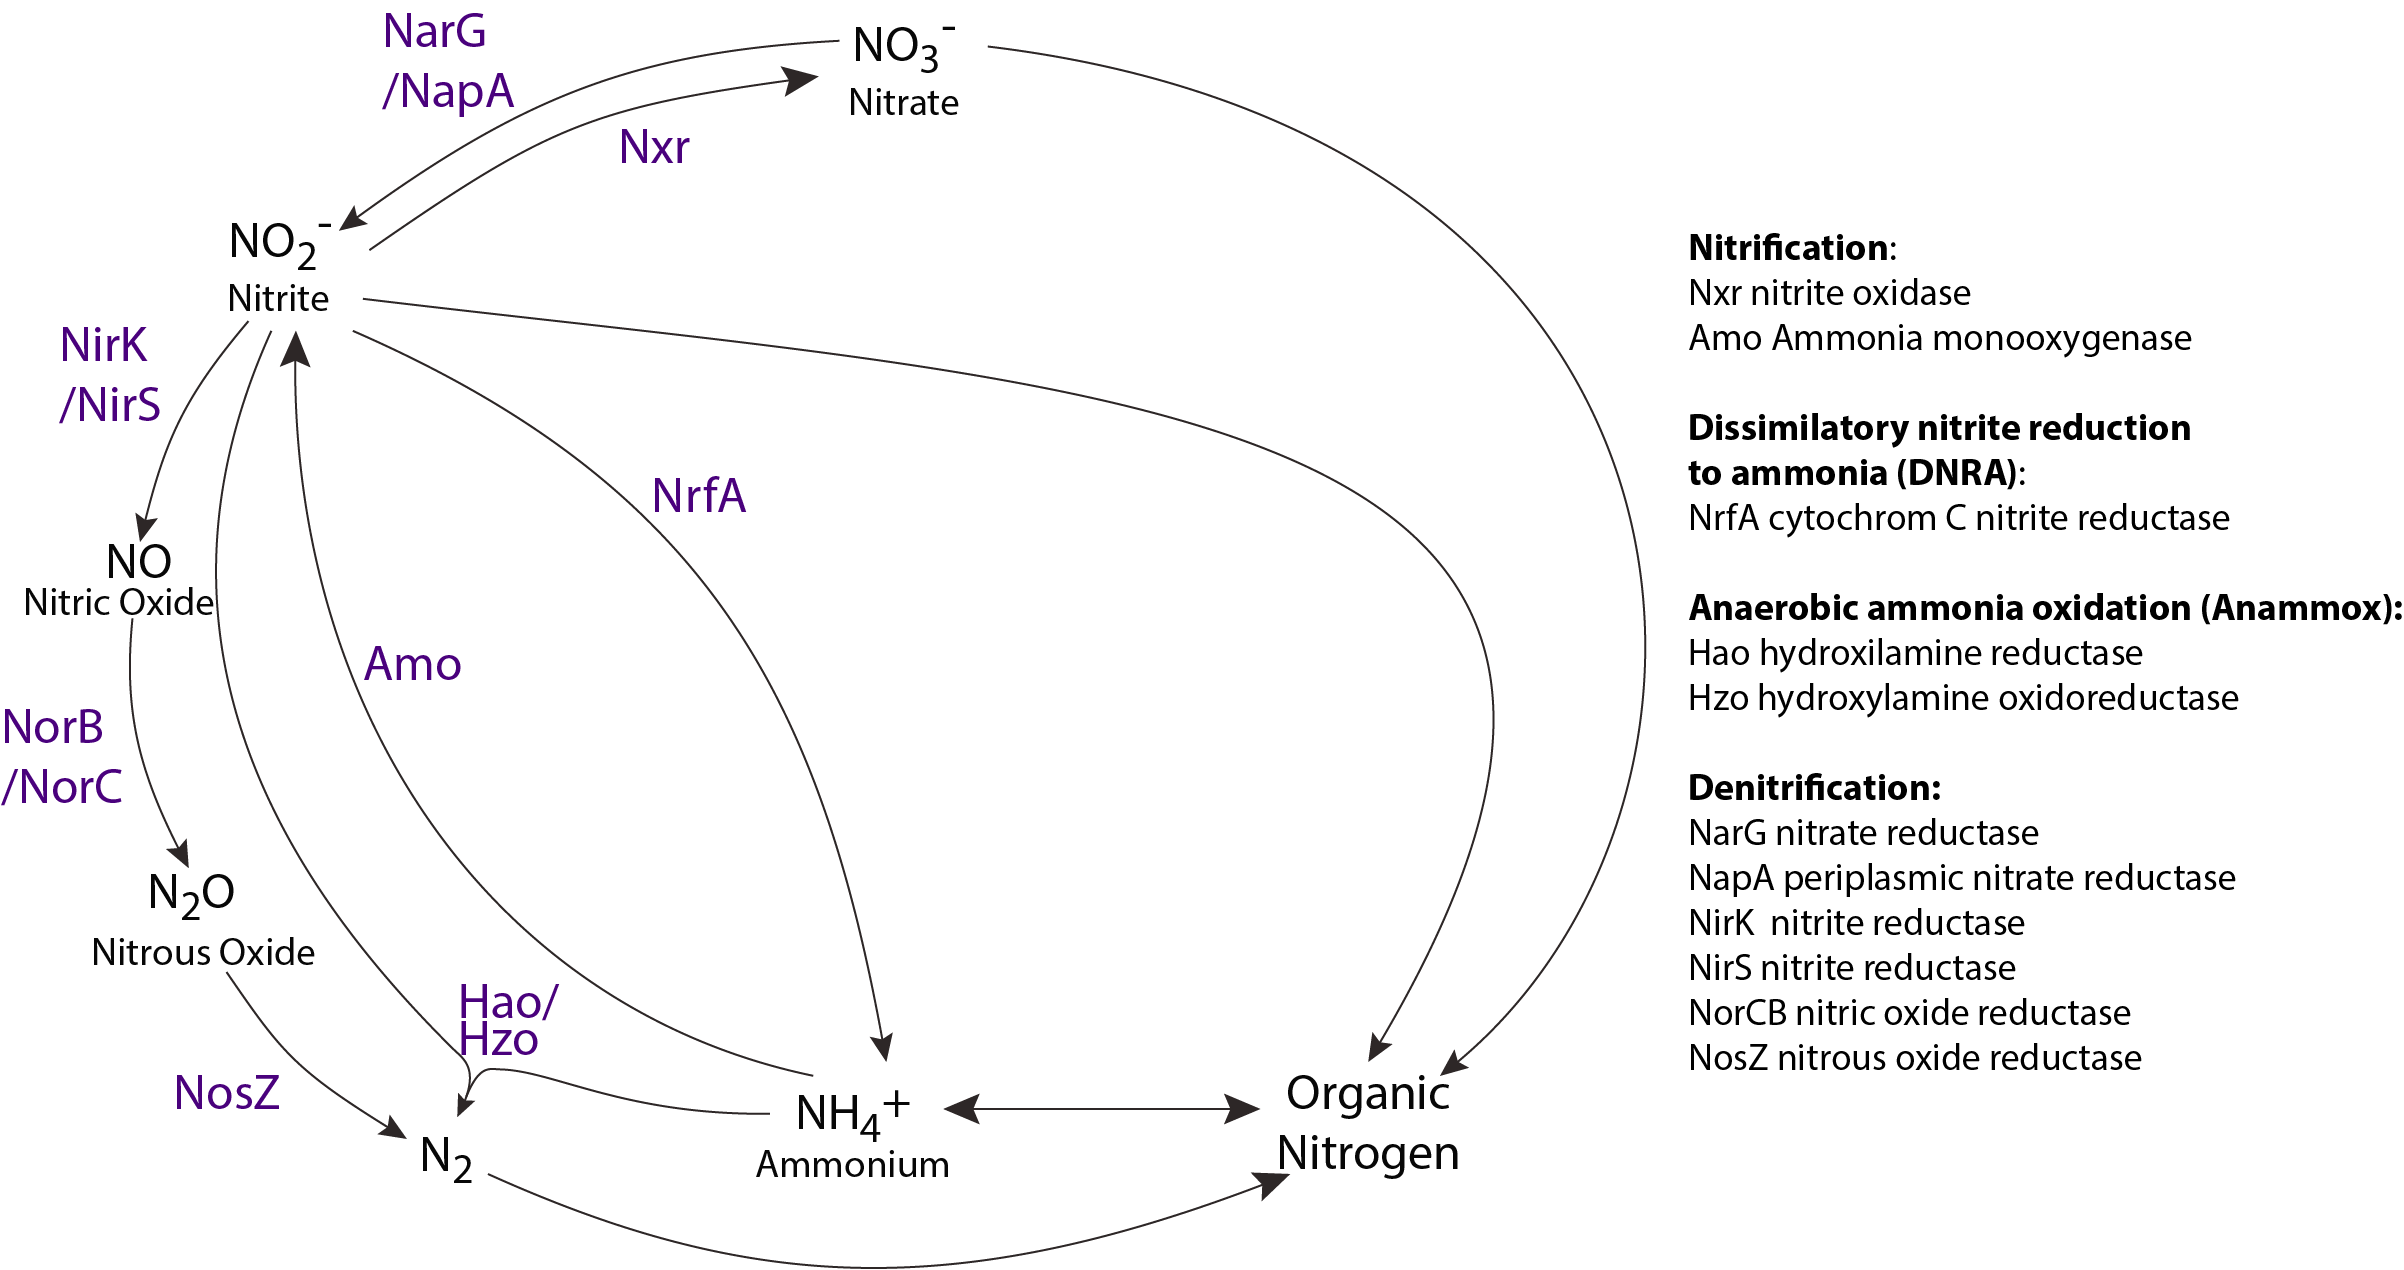
\includegraphics{N_Cycle_Figure.png}
\caption{Figure 1: Nitrogen Cycle}
\end{figure}

The denitrification process plays an integral role in the global
nitrogen balance. It returns the nitrogen into the atmosphere and
maintains homeostasis between the nitrogen content of soil and air. (8).
The four enzymes of denitrification are: nitrate, nitrite, nitric oxide
and nitrous oxide reductase which are encoded by \emph{nar}, \emph{nir},
\emph{nor}, and \emph{nos}, respectively (9). Denitrification takes
place in aquatic, marine, and terrestrial ecosystems, and the rate of
this process is affected by various factors such as pH, temperature, and
oxygen concentration (8). In OMZs, nitrate
(NO\textsubscript{3}\textsuperscript{-}) and nitrite
(NO\textsubscript{2}\textsuperscript{-}) act as the main terminal
electron acceptors in respiration (10). Nitrogen oxide reductases are
sensitive to oxygen and it is known that oxygen represses
denitrification (8). Among the four N-oxide reductases, nitrous oxide
reductase is the most sensitive enzyme to oxygen, leading to the
increase in N\textsubscript{2}O production in the suboxic and anoxic
conditions (10). The interest in denitrification process is for several
reasons. Denitrification is the process contributing to the loss of
fertilizer nitrogen, therefore reducing the agriculture productivity
(7). Additionally, denitrification can be utilized to remove nitrogen
from high-nitrate wastewaters to decrease the contamination and
eutrophication (7). However, denitrification can have negative effects
on the climate system, as the emission of N\textsubscript{2}O leads to
stratospheric ozone layer depletion, contributing to global warming (7).
Some of the major denitrifying bacteria are from genera:
\emph{Alcaligenes}, \emph{Agrobacterium}, \emph{Bacillus},
\emph{Hyphomicrobium}, \emph{Moraxella}, \emph{Pseudomonas}, and
\emph{Paracoccus} (7). Due to the high frequency of isolation, the
genera \emph{Pseudomonas} and \emph{Alcaligenes} are of the greatest
significance (4).

The objective of this project is to reassemble the nitrogen cycle as a
distributed metabolic process which may provide new insight into the
roles that microbes play on nutrient and energy fluxes in the ocean.
There are several well-defined gene encoding key steps in the nitrogen
cycle and they serve as basis for functional anchor screening to
determine their distribution across the Tree of Life. Here, we focused
on the nitric oxide reductase, \emph{norB}, and we examined its DNA and
RNA abundance across the different depths in Saanich Inlet. We also
investigated how the nitrogen species in Saanich relate to the
abundances of \emph{norB}.

\section{Materials and Experimental
Configuration}\label{materials-and-experimental-configuration}

\subsection{Methods}\label{methods}

\begin{Shaded}
\begin{Highlighting}[]
\NormalTok{## DNA}
\NormalTok{norB.DNA.10m <-}\StringTok{ }\KeywordTok{read_tsv}\NormalTok{(}\StringTok{"data/dna/norB_DNA_10m_marker_contig_map.tsv"}\NormalTok{) }\OperatorTok\StringTok{ }
\StringTok{    }\KeywordTok{select}\NormalTok{(}\DataTypeTok{Tax.DNA.10 =}\NormalTok{ Confident_Taxonomy, }\DataTypeTok{Abund.DNA.10 =}\NormalTok{ Abundance, Query)}

\NormalTok{norB.DNA.100m <-}\StringTok{ }\KeywordTok{read_tsv}\NormalTok{(}\StringTok{"data/dna/norB_DNA_100m_marker_contig_map.tsv"}\NormalTok{) }\OperatorTok\StringTok{ }
\StringTok{    }\KeywordTok{select}\NormalTok{(}\DataTypeTok{Tax.DNA.100 =}\NormalTok{ Confident_Taxonomy, }\DataTypeTok{Abund.DNA.100 =}\NormalTok{ Abundance, Query)}

\NormalTok{norB.DNA.120m <-}\StringTok{ }\KeywordTok{read_tsv}\NormalTok{(}\StringTok{"data/dna/norB_DNA_120m_marker_contig_map.tsv"}\NormalTok{) }\OperatorTok\StringTok{ }
\StringTok{    }\KeywordTok{select}\NormalTok{(}\DataTypeTok{Tax.DNA.120 =}\NormalTok{ Confident_Taxonomy, }\DataTypeTok{Abund.DNA.120 =}\NormalTok{ Abundance, Query)}

\NormalTok{norB.DNA.135m <-}\StringTok{ }\KeywordTok{read_tsv}\NormalTok{(}\StringTok{"data/dna/norB_DNA_135m_marker_contig_map.tsv"}\NormalTok{) }\OperatorTok\StringTok{ }
\StringTok{    }\KeywordTok{select}\NormalTok{(}\DataTypeTok{Tax.DNA.135 =}\NormalTok{ Confident_Taxonomy, }\DataTypeTok{Abund.DNA.135 =}\NormalTok{ Abundance, Query)}

\NormalTok{norB.DNA.150m <-}\StringTok{ }\KeywordTok{read_tsv}\NormalTok{(}\StringTok{"data/dna/norB_DNA_150m_marker_contig_map.tsv"}\NormalTok{) }\OperatorTok\StringTok{ }
\StringTok{    }\KeywordTok{select}\NormalTok{(}\DataTypeTok{Tax.DNA.150 =}\NormalTok{ Confident_Taxonomy, }\DataTypeTok{Abund.DNA.150 =}\NormalTok{ Abundance, Query)}

\NormalTok{norB.DNA.165m <-}\StringTok{ }\KeywordTok{read_tsv}\NormalTok{(}\StringTok{"data/dna/norB_DNA_165m_marker_contig_map.tsv"}\NormalTok{) }\OperatorTok\StringTok{ }
\StringTok{    }\KeywordTok{select}\NormalTok{(}\DataTypeTok{Tax.DNA.165 =}\NormalTok{ Confident_Taxonomy, }\DataTypeTok{Abund.DNA.165 =}\NormalTok{ Abundance, Query)}

\NormalTok{norB.DNA.200m <-}\StringTok{ }\KeywordTok{read_tsv}\NormalTok{(}\StringTok{"data/dna/norB_DNA_200m_marker_contig_map.tsv"}\NormalTok{) }\OperatorTok\StringTok{ }
\StringTok{    }\KeywordTok{select}\NormalTok{(}\DataTypeTok{Tax.DNA.200 =}\NormalTok{ Confident_Taxonomy, }\DataTypeTok{Abund.DNA.200 =}\NormalTok{ Abundance, Query)}

\NormalTok{## RNA}
\NormalTok{norB.RNA.10m <-}\StringTok{ }\KeywordTok{read_tsv}\NormalTok{(}\StringTok{"data/rna/norB_RNA_10m_marker_contig_map.tsv"}\NormalTok{) }\OperatorTok\StringTok{ }
\StringTok{    }\KeywordTok{select}\NormalTok{(}\DataTypeTok{Tax.RNA.10 =}\NormalTok{ Confident_Taxonomy, }\DataTypeTok{Abund.RNA.10 =}\NormalTok{ Abundance, Query)}

\NormalTok{norB.RNA.100m <-}\StringTok{ }\KeywordTok{read_tsv}\NormalTok{(}\StringTok{"data/rna/norB_RNA_100m_marker_contig_map.tsv"}\NormalTok{) }\OperatorTok\StringTok{ }
\StringTok{    }\KeywordTok{select}\NormalTok{(}\DataTypeTok{Tax.RNA.100 =}\NormalTok{ Confident_Taxonomy, }\DataTypeTok{Abund.RNA.100 =}\NormalTok{ Abundance, Query)}

\NormalTok{norB.RNA.120m <-}\StringTok{ }\KeywordTok{read_tsv}\NormalTok{(}\StringTok{"data/rna/norB_RNA_120m_marker_contig_map.tsv"}\NormalTok{) }\OperatorTok\StringTok{ }
\StringTok{    }\KeywordTok{select}\NormalTok{(}\DataTypeTok{Tax.RNA.120 =}\NormalTok{ Confident_Taxonomy, }\DataTypeTok{Abund.RNA.120 =}\NormalTok{ Abundance, Query)}

\NormalTok{norB.RNA.135m <-}\StringTok{ }\KeywordTok{read_tsv}\NormalTok{(}\StringTok{"data/rna/norB_RNA_135m_marker_contig_map.tsv"}\NormalTok{) }\OperatorTok\StringTok{ }
\StringTok{    }\KeywordTok{select}\NormalTok{(}\DataTypeTok{Tax.RNA.135 =}\NormalTok{ Confident_Taxonomy, }\DataTypeTok{Abund.RNA.135 =}\NormalTok{ Abundance, Query)}

\NormalTok{norB.RNA.150m <-}\StringTok{ }\KeywordTok{read_tsv}\NormalTok{(}\StringTok{"data/rna/norB_RNA_150m_marker_contig_map.tsv"}\NormalTok{) }\OperatorTok\StringTok{ }
\StringTok{    }\KeywordTok{select}\NormalTok{(}\DataTypeTok{Tax.RNA.150 =}\NormalTok{ Confident_Taxonomy, }\DataTypeTok{Abund.RNA.150 =}\NormalTok{ Abundance, Query)}

\NormalTok{norB.RNA.165m <-}\StringTok{ }\KeywordTok{read_tsv}\NormalTok{(}\StringTok{"data/rna/norB_RNA_165m_marker_contig_map.tsv"}\NormalTok{) }\OperatorTok\StringTok{ }
\StringTok{    }\KeywordTok{select}\NormalTok{(}\DataTypeTok{Tax.RNA.165 =}\NormalTok{ Confident_Taxonomy, }\DataTypeTok{Abund.RNA.165 =}\NormalTok{ Abundance, Query)}

\NormalTok{norB.RNA.200m <-}\StringTok{ }\KeywordTok{read_tsv}\NormalTok{(}\StringTok{"data/rna/norB_RNA_200m_marker_contig_map.tsv"}\NormalTok{) }\OperatorTok\StringTok{ }
\StringTok{    }\KeywordTok{select}\NormalTok{(}\DataTypeTok{Tax.RNA.200 =}\NormalTok{ Confident_Taxonomy, }\DataTypeTok{Abund.RNA.200 =}\NormalTok{ Abundance, Query)}
\end{Highlighting}
\end{Shaded}

\begin{Shaded}
\begin{Highlighting}[]
\NormalTok{norB.all <-}\StringTok{ }\NormalTok{norB.DNA.10m }\OperatorTok\StringTok{ }\CommentTok{# Combine the data frames will full_join to keep all the data}
\KeywordTok{full_join}\NormalTok{(norB.DNA.100m, }\DataTypeTok{by =} \StringTok{"Query"}\NormalTok{) }\OperatorTok\StringTok{ }\KeywordTok{full_join}\NormalTok{(norB.DNA.120m, }\DataTypeTok{by =} \StringTok{"Query"}\NormalTok{) }\OperatorTok\StringTok{ }
\StringTok{    }\KeywordTok{full_join}\NormalTok{(norB.DNA.135m, }\DataTypeTok{by =} \StringTok{"Query"}\NormalTok{) }\OperatorTok\StringTok{ }\KeywordTok{full_join}\NormalTok{(norB.DNA.150m, }\DataTypeTok{by =} \StringTok{"Query"}\NormalTok{) }\OperatorTok\StringTok{ }
\StringTok{    }\KeywordTok{full_join}\NormalTok{(norB.DNA.165m, }\DataTypeTok{by =} \StringTok{"Query"}\NormalTok{) }\OperatorTok\StringTok{ }\KeywordTok{full_join}\NormalTok{(norB.DNA.200m, }\DataTypeTok{by =} \StringTok{"Query"}\NormalTok{) }\OperatorTok\StringTok{ }
\StringTok{    }\KeywordTok{full_join}\NormalTok{(norB.RNA.10m, }\DataTypeTok{by =} \StringTok{"Query"}\NormalTok{) }\OperatorTok\StringTok{ }\KeywordTok{full_join}\NormalTok{(norB.RNA.100m, }\DataTypeTok{by =} \StringTok{"Query"}\NormalTok{) }\OperatorTok\StringTok{ }
\StringTok{    }\KeywordTok{full_join}\NormalTok{(norB.RNA.120m, }\DataTypeTok{by =} \StringTok{"Query"}\NormalTok{) }\OperatorTok\StringTok{ }\KeywordTok{full_join}\NormalTok{(norB.RNA.135m, }\DataTypeTok{by =} \StringTok{"Query"}\NormalTok{) }\OperatorTok\StringTok{ }
\StringTok{    }\KeywordTok{full_join}\NormalTok{(norB.RNA.150m, }\DataTypeTok{by =} \StringTok{"Query"}\NormalTok{) }\OperatorTok\StringTok{ }\KeywordTok{full_join}\NormalTok{(norB.RNA.165m, }\DataTypeTok{by =} \StringTok{"Query"}\NormalTok{) }\OperatorTok\StringTok{ }
\StringTok{    }\KeywordTok{full_join}\NormalTok{(norB.RNA.200m, }\DataTypeTok{by =} \StringTok{"Query"}\NormalTok{) }\OperatorTok\StringTok{ }\CommentTok{# Create a taxonomy variable aggregating all taxonomy columns so as to fill}
\CommentTok{# in any NAs that might occur. !is.na means 'is not NA', so the following}
\CommentTok{# says that the Taxonomy data should be taken from Tax.RNA.10 if that is not}
\CommentTok{# NA, or else take it from Tax.DNA.10 if that is not NA, or else}
\CommentTok{# Tax.RNA.200, etc. until if all are NA, give Taxonomy of 'unclassified'}
\KeywordTok{mutate}\NormalTok{(}\DataTypeTok{Taxonomy =} \KeywordTok{ifelse}\NormalTok{(}\OperatorTok{!}\KeywordTok{is.na}\NormalTok{(Tax.DNA.}\DecValTok{10}\NormalTok{), Tax.DNA.}\DecValTok{10}\NormalTok{, }\KeywordTok{ifelse}\NormalTok{(}\OperatorTok{!}\KeywordTok{is.na}\NormalTok{(Tax.DNA.}\DecValTok{100}\NormalTok{), }
\NormalTok{    Tax.DNA.}\DecValTok{100}\NormalTok{, }\KeywordTok{ifelse}\NormalTok{(}\OperatorTok{!}\KeywordTok{is.na}\NormalTok{(Tax.DNA.}\DecValTok{120}\NormalTok{), Tax.DNA.}\DecValTok{120}\NormalTok{, }\KeywordTok{ifelse}\NormalTok{(}\OperatorTok{!}\KeywordTok{is.na}\NormalTok{(Tax.DNA.}\DecValTok{135}\NormalTok{), }
\NormalTok{        Tax.DNA.}\DecValTok{135}\NormalTok{, }\KeywordTok{ifelse}\NormalTok{(}\OperatorTok{!}\KeywordTok{is.na}\NormalTok{(Tax.DNA.}\DecValTok{150}\NormalTok{), Tax.DNA.}\DecValTok{150}\NormalTok{, }\KeywordTok{ifelse}\NormalTok{(}\OperatorTok{!}\KeywordTok{is.na}\NormalTok{(Tax.DNA.}\DecValTok{165}\NormalTok{), }
\NormalTok{            Tax.DNA.}\DecValTok{165}\NormalTok{, }\KeywordTok{ifelse}\NormalTok{(}\OperatorTok{!}\KeywordTok{is.na}\NormalTok{(Tax.DNA.}\DecValTok{200}\NormalTok{), Tax.DNA.}\DecValTok{200}\NormalTok{, }\KeywordTok{ifelse}\NormalTok{(}\OperatorTok{!}\KeywordTok{is.na}\NormalTok{(Tax.RNA.}\DecValTok{10}\NormalTok{), }
\NormalTok{                Tax.RNA.}\DecValTok{10}\NormalTok{, }\KeywordTok{ifelse}\NormalTok{(}\OperatorTok{!}\KeywordTok{is.na}\NormalTok{(Tax.RNA.}\DecValTok{100}\NormalTok{), Tax.RNA.}\DecValTok{100}\NormalTok{, }\KeywordTok{ifelse}\NormalTok{(}\OperatorTok{!}\KeywordTok{is.na}\NormalTok{(Tax.RNA.}\DecValTok{120}\NormalTok{), }
\NormalTok{                  Tax.RNA.}\DecValTok{120}\NormalTok{, }\KeywordTok{ifelse}\NormalTok{(}\OperatorTok{!}\KeywordTok{is.na}\NormalTok{(Tax.RNA.}\DecValTok{135}\NormalTok{), Tax.RNA.}\DecValTok{135}\NormalTok{, }\KeywordTok{ifelse}\NormalTok{(}\OperatorTok{!}\KeywordTok{is.na}\NormalTok{(Tax.RNA.}\DecValTok{150}\NormalTok{), }
\NormalTok{                    Tax.RNA.}\DecValTok{150}\NormalTok{, }\KeywordTok{ifelse}\NormalTok{(}\OperatorTok{!}\KeywordTok{is.na}\NormalTok{(Tax.RNA.}\DecValTok{165}\NormalTok{), Tax.RNA.}\DecValTok{165}\NormalTok{, }\KeywordTok{ifelse}\NormalTok{(}\OperatorTok{!}\KeywordTok{is.na}\NormalTok{(Tax.RNA.}\DecValTok{200}\NormalTok{), }
\NormalTok{                      Tax.RNA.}\DecValTok{200}\NormalTok{, }\StringTok{"unclassified"}\NormalTok{))))))))))))))) }\OperatorTok\StringTok{ }\CommentTok{# Get rid of the old Tax variables}
\KeywordTok{select}\NormalTok{(}\OperatorTok{-}\KeywordTok{starts_with}\NormalTok{(}\StringTok{"Tax."}\NormalTok{)) }\OperatorTok\StringTok{ }\CommentTok{# Gather all the abundance data into 1 column}
\KeywordTok{gather}\NormalTok{(}\StringTok{"Key"}\NormalTok{, }\StringTok{"Abundance"}\NormalTok{, }\KeywordTok{starts_with}\NormalTok{(}\StringTok{"Abund"}\NormalTok{)) }\OperatorTok\StringTok{ }\CommentTok{# Turn the Key into Depth and RNA/DNA variables. We can easily do this}
\CommentTok{# because we specifically named these variables with period separation when}
\CommentTok{# we loaded in the original data}
\KeywordTok{separate}\NormalTok{(Key, }\KeywordTok{c}\NormalTok{(}\StringTok{"Key"}\NormalTok{, }\StringTok{"Type"}\NormalTok{, }\StringTok{"Depth_m"}\NormalTok{), }\DataTypeTok{by =} \StringTok{"."}\NormalTok{) }\OperatorTok\StringTok{ }\CommentTok{# Remove Key variable now that it only contains 'Abund'. This also serves to}
\CommentTok{# reorder the columns so that the very long Query is at the end.}
\KeywordTok{select}\NormalTok{(Depth_m, Type, Abundance, Taxonomy, Query) }\OperatorTok\StringTok{ }\CommentTok{# Make sure R knows depth is numerical since it came from a character}
\CommentTok{# variable}
\KeywordTok{mutate}\NormalTok{(}\DataTypeTok{Depth_m =} \KeywordTok{as.numeric}\NormalTok{(Depth_m)) }\OperatorTok\StringTok{ }\CommentTok{# Make sure to impute missing abundant information by setting it to 0}
\KeywordTok{mutate}\NormalTok{(}\DataTypeTok{Abundance =} \KeywordTok{ifelse}\NormalTok{(}\KeywordTok{is.na}\NormalTok{(Abundance), }\DecValTok{0}\NormalTok{, Abundance)) }\OperatorTok\StringTok{ }\CommentTok{# Separate Taxonomy into columns so we can plot at different levels}
\KeywordTok{separate}\NormalTok{(Taxonomy, }\DataTypeTok{into =} \KeywordTok{c}\NormalTok{(}\StringTok{"Domain"}\NormalTok{, }\StringTok{"Phylum"}\NormalTok{, }\StringTok{"Class"}\NormalTok{, }\StringTok{"Order"}\NormalTok{, }\StringTok{"Family"}\NormalTok{, }
    \StringTok{"Genus"}\NormalTok{, }\StringTok{"Species"}\NormalTok{), }\DataTypeTok{sep =} \StringTok{"; "}\NormalTok{)}

\NormalTok{norB.all.norm <-}\StringTok{ }\NormalTok{norB.all}
\end{Highlighting}
\end{Shaded}

Sequences for \emph{norB} were obtained from various depths at Saanich
Inlet. Listed below are the method of processing the tree-based
sensitive and accurate protein profiler (TreeSAPP):

\begin{enumerate}
\def\labelenumi{\arabic{enumi})}
\tightlist
\item
  The query sequences were first mapped to the reference sequences in
  BLASTp.
\item
  Coding sequences were then extracted and queried with putative
  functions
\item
  Profile-alignment (HmmAlign) with multiple alignment of references and
  query
\item
  Classification of sequence insertions were then done in reference
  trees (RAxML)
\item
  Reference trees were then updated with novel sequences
\item
  Construction of trees at various depths with Interactive Tree of Life
  (iTOL)
\end{enumerate}

Majority of TreeSAPP pipeline was run on Google Cloud for metagenomic
(MetaG, DNA) and metatranscriptomic (MetaT, RNA) assemblies of norB gene
at the depths of 10m, 100m, 120m, 135m, 150m, 165m, and 200m. Reads per
kilo base per million mapped reads (RPKM) was used for normalization
when comparing the gene converage values, which corrected differences in
sampling sequencing depth and gene length (16). The formula used in RPKM
is indicated below:

RPKM = numReads / (geneLength/1000 * totalNumReads/1,000,000)

Where numReads was the number of reads mapped to a gene sequence,
geneLength was the length of the gene sequence, and totalNumReads was
the total number of mapped reads of a sample.

The following codes below were used in the pipeline (15). More
information can be obtained from the TreeSAPP Demo on Github:

time treesapp.py -T 8 --verbose --delete --pairing pe\\
Various functions were stated with the following line above for:
Tracking the runtime, specifying the maximum number of threads (8) to be
used for efficiency, printing the intermediate steps, deleting the
intermediate files to reduce the storage space occupied, and lastly
specifying the usage of paired end files for comparing our data.

-t D0501\\
Target gene was specified here (D0501, which corresponded to
\emph{norB}).

-i bucket/MetaG\_assemblies/depth\#\_assembly.fasta --rpkm\\
Input files and path to store files was specified with the following
line above.

-r bucket/MetaG\_reads/depth\#.fastq.gz\\
The input files for MetaG and MetaT reads were also specified above.

-o treesapp\_out\_dir\_depth\#\\
Output file name was specified above.

rm treesapp\_out\_dir\_depth1/RPKM\_outputs/*.sam\\
Last instruction here was used to remove gigabyte size intermediate SAM
files.

Visualization of output files at various depths were done on iTOL v4 for
\emph{norB} gene.

Using the processed results, DNA abundance and RNA abundance analyses
were done for \emph{norB} at multiple depths (Fig. 2 and Fig. 3). In
addition, various genera were also compared in regards to their DNA
vs.~RNA abundances to determine the expression of \emph{norB} for each
genus at different depths (Fig. 4a and Fib 4b). Lastly, the relationship
of abundance of \emph{norB} and concentration of several nitrogen
species – such as nitrate, nitrogen dioxide, and nitrous oxide –
were also observed (Fig. 5).

\section{Results}\label{results}

\subsection{\texorpdfstring{Analysis of the DNA abundance of \emph{norB}
with
depth}{Analysis of the DNA abundance of norB with depth}}\label{analysis-of-the-dna-abundance-of-norb-with-depth}

\begin{Shaded}
\begin{Highlighting}[]
\NormalTok{abun.dna.by.depth <-}\StringTok{ }\NormalTok{norB.all }\OperatorTok\StringTok{ }\KeywordTok{filter}\NormalTok{(Type }\OperatorTok{==}\StringTok{ "DNA"}\NormalTok{) }\OperatorTok\StringTok{ }\KeywordTok{group_by}\NormalTok{(Depth_m) }\OperatorTok\StringTok{ }
\StringTok{    }\KeywordTok{summarise}\NormalTok{(}\DataTypeTok{Abundance_DNA =} \KeywordTok{sum}\NormalTok{(Abundance))}

\KeywordTok{kable}\NormalTok{(abun.dna.by.depth, }\DataTypeTok{caption =} \StringTok{"Table 1: Abundance of the norB gene (DNA) at different depths by RPKM"}\NormalTok{)}
\end{Highlighting}
\end{Shaded}

\begin{longtable}[]{@{}rr@{}}
\caption{Table 1: Abundance of the norB gene (DNA) at different depths
by RPKM}\tabularnewline
\toprule
Depth\_m & Abundance\_DNA\tabularnewline
\midrule
\endfirsthead
\toprule
Depth\_m & Abundance\_DNA\tabularnewline
\midrule
\endhead
10 & 1.581131\tabularnewline
100 & 101.397580\tabularnewline
120 & 197.248612\tabularnewline
135 & 345.156101\tabularnewline
150 & 541.756037\tabularnewline
165 & 137.576279\tabularnewline
200 & 854.085568\tabularnewline
\bottomrule
\end{longtable}

\begin{Shaded}
\begin{Highlighting}[]
\NormalTok{plot1 <-}\StringTok{ }\NormalTok{norB.all.norm }\OperatorTok\StringTok{ }\CommentTok{# Filter the DNA data}
\KeywordTok{filter}\NormalTok{(Type }\OperatorTok{==}\StringTok{ "DNA"}\NormalTok{) }\OperatorTok\StringTok{ }\CommentTok{# Change NAs to 'unclassified' at the level you want to plot. Here we will}
\CommentTok{# do Genus}
\KeywordTok{mutate}\NormalTok{(}\DataTypeTok{Genus =} \KeywordTok{ifelse}\NormalTok{(}\KeywordTok{is.na}\NormalTok{(Genus), }\StringTok{"unclassified"}\NormalTok{, Genus)) }\OperatorTok\StringTok{ }
\KeywordTok{ggplot}\NormalTok{(}\KeywordTok{aes}\NormalTok{(}\DataTypeTok{x =} \StringTok{"norB"}\NormalTok{, }\DataTypeTok{y =}\NormalTok{ Depth_m)) }\OperatorTok{+}\StringTok{ }\CommentTok{# Use the size aesthetic to show abundance}
\KeywordTok{geom_point}\NormalTok{(}\KeywordTok{aes}\NormalTok{(}\DataTypeTok{size =} \KeywordTok{ifelse}\NormalTok{(Abundance }\OperatorTok{==}\StringTok{ }\DecValTok{0}\NormalTok{, }\OtherTok{NA}\NormalTok{, Abundance)), }\DataTypeTok{colour =} \StringTok{"brown"}\NormalTok{) }\OperatorTok{+}\StringTok{ }
\StringTok{    }\CommentTok{# Reverse the why axis so depth increases going down}
\KeywordTok{scale_y_reverse}\NormalTok{(}\DataTypeTok{lim =} \KeywordTok{c}\NormalTok{(}\DecValTok{200}\NormalTok{, }\DecValTok{10}\NormalTok{)) }\OperatorTok{+}\StringTok{ }\KeywordTok{scale_size}\NormalTok{(}\StringTok{"Abundance"}\NormalTok{) }\OperatorTok{+}\StringTok{ }\KeywordTok{labs}\NormalTok{(}\DataTypeTok{x =} \StringTok{""}\NormalTok{, }\DataTypeTok{y =} \StringTok{"Depth (m)"}\NormalTok{) }\OperatorTok{+}\StringTok{ }
\StringTok{    }\KeywordTok{theme_classic}\NormalTok{()}

\KeywordTok{annotate_figure}\NormalTok{(plot1, }\DataTypeTok{bottom =} \KeywordTok{text_grob}\NormalTok{(}\StringTok{"Figure 2: Abundance (0-1) of norB gene (DNA) at different depths"}\NormalTok{, }
    \DataTypeTok{size =} \DecValTok{12}\NormalTok{))}
\end{Highlighting}
\end{Shaded}

\begin{center}\includegraphics{main_files/figure-latex/figure2-1} \end{center}

In Fig. 2, the DNA abundance of \emph{norB} followed an upwards trend
where it increased from 50 at depth 100m to 200 at depth 200m. This was
consistent with what had been shown in previous studies, where genes
associated with partial denitrification to nitrous oxide were most
abundant at a depth of 150m and were not present at depth 50m (11). An
exception of this trend occurs at depth 165m, where DNA abundance
declined sharply to 50 as shown in Figure 2. This decline can be
attributed to the low abundance of \emph{norB} DNA of Proteobacteria at
depth 165m (Fig. 4). A comparison of Fig. 2 and Fig. 4 reveals that the
DNA abundance of \emph{norB} gene mostly reflects \emph{norB} DNA
abundance of Proteobacteria. This suggested that the Proteobacteria
phylum is the major contributor to the DNA abundance of \emph{norB}
gene.

\subsection{\texorpdfstring{Analysis of similarities between RNA and DNA
abundance information of \emph{norB} with
depths}{Analysis of similarities between RNA and DNA abundance information of norB with depths}}\label{analysis-of-similarities-between-rna-and-dna-abundance-information-of-norb-with-depths}

\begin{Shaded}
\begin{Highlighting}[]
\NormalTok{abun.rna.by.depth <-}\StringTok{ }\NormalTok{norB.all }\OperatorTok\StringTok{ }\KeywordTok{filter}\NormalTok{(Type }\OperatorTok{==}\StringTok{ "RNA"}\NormalTok{) }\OperatorTok\StringTok{ }\KeywordTok{group_by}\NormalTok{(Depth_m) }\OperatorTok\StringTok{ }
\StringTok{    }\KeywordTok{summarise}\NormalTok{(}\DataTypeTok{Abundance_RNA =} \KeywordTok{sum}\NormalTok{(Abundance))}

\NormalTok{abun.by.depth <-}\StringTok{ }\KeywordTok{full_join}\NormalTok{(}\DataTypeTok{x =}\NormalTok{ abun.dna.by.depth, }\DataTypeTok{y =}\NormalTok{ abun.rna.by.depth, }\DataTypeTok{by =} \StringTok{"Depth_m"}\NormalTok{)}
\KeywordTok{kable}\NormalTok{(abun.by.depth, }\DataTypeTok{caption =} \StringTok{"Table 2: Abundance of norB gene (DNA vs. RNA) at different depths by RPKM"}\NormalTok{)}
\end{Highlighting}
\end{Shaded}

\begin{longtable}[]{@{}rrr@{}}
\caption{Table 2: Abundance of norB gene (DNA vs.~RNA) at different
depths by RPKM}\tabularnewline
\toprule
Depth\_m & Abundance\_DNA & Abundance\_RNA\tabularnewline
\midrule
\endfirsthead
\toprule
Depth\_m & Abundance\_DNA & Abundance\_RNA\tabularnewline
\midrule
\endhead
10 & 1.581131 & 0.000000\tabularnewline
100 & 101.397580 & 4.256517\tabularnewline
120 & 197.248612 & 8.066146\tabularnewline
135 & 345.156101 & 55.932741\tabularnewline
150 & 541.756037 & 788.040985\tabularnewline
165 & 137.576279 & 912.117306\tabularnewline
200 & 854.085568 & 944.915908\tabularnewline
\bottomrule
\end{longtable}

\begin{Shaded}
\begin{Highlighting}[]
\NormalTok{plot1 <-}\StringTok{ }\NormalTok{norB.all.norm }\OperatorTok\StringTok{ }\CommentTok{# Change NAs to 'unclassified' at the level you want to plot}
\KeywordTok{mutate}\NormalTok{(}\DataTypeTok{Genus =} \KeywordTok{ifelse}\NormalTok{(}\KeywordTok{is.na}\NormalTok{(Genus), }\StringTok{"unclassified"}\NormalTok{, Genus)) }\OperatorTok\StringTok{ }\KeywordTok{group_by}\NormalTok{(Depth_m) }\OperatorTok\StringTok{ }
\StringTok{    }\CommentTok{# Show both RNA and DNA using an x variable}
\KeywordTok{ggplot}\NormalTok{(}\KeywordTok{aes}\NormalTok{(}\DataTypeTok{x =}\NormalTok{ Type, }\DataTypeTok{y =}\NormalTok{ Depth_m)) }\OperatorTok{+}\StringTok{ }\KeywordTok{geom_point}\NormalTok{(}\KeywordTok{aes}\NormalTok{(}\DataTypeTok{size =} \KeywordTok{ifelse}\NormalTok{(Abundance }\OperatorTok{==}\StringTok{ }
\StringTok{    }\DecValTok{0}\NormalTok{, }\OtherTok{NA}\NormalTok{, Abundance))) }\OperatorTok{+}\StringTok{ }\KeywordTok{geom_point}\NormalTok{(}\DataTypeTok{shape =} \DecValTok{21}\NormalTok{) }\OperatorTok{+}\StringTok{ }\KeywordTok{scale_y_reverse}\NormalTok{(}\DataTypeTok{lim =} \KeywordTok{c}\NormalTok{(}\DecValTok{200}\NormalTok{, }
    \DecValTok{10}\NormalTok{)) }\OperatorTok{+}\StringTok{ }\CommentTok{# Remove zeros by setting min limit to 1e-09}
\KeywordTok{scale_size}\NormalTok{(}\StringTok{"Abundance"}\NormalTok{) }\OperatorTok{+}\StringTok{ }\KeywordTok{labs}\NormalTok{(}\DataTypeTok{x =} \StringTok{""}\NormalTok{, }\DataTypeTok{y =} \StringTok{"Depth (m)"}\NormalTok{) }\OperatorTok{+}\StringTok{ }\KeywordTok{theme_classic}\NormalTok{()}

\KeywordTok{annotate_figure}\NormalTok{(plot1, }\DataTypeTok{bottom =} \KeywordTok{text_grob}\NormalTok{(}\StringTok{"Figure 3: Abundance (0-1) of norB gene (DNA vs. RNA) at different depths"}\NormalTok{, }
    \DataTypeTok{size =} \DecValTok{12}\NormalTok{))}
\end{Highlighting}
\end{Shaded}

\begin{center}\includegraphics{main_files/figure-latex/figure3-1} \end{center}

It was observed that the RNA abundance of \emph{norB} gene in Fig. 3
followed a similar linear trend as the DNA abundance in Fig. 2. The
abundance of RNA increased from around 30 at depth 100m to 500 at depth
200m (Fig. 3). However, the sharp decrease in DNA abundance at 165m
depth was not observed for the RNA abundance of \emph{norB} gene. In
Fig. 4, the trend for RNA abundance of \emph{norB} gene follows the same
trend as the \emph{norB} RNA abundance of the Proteobacteria phylum.
This demonstrated that despite the low abundance of \emph{norB} DNA at
depth 165m, the expression of gene is high leading to an increase in the
amount of \emph{norB} RNA that is observed.

\subsection{Reconstructing the associated taxa with norB and analyze
variances of DNA and RNA based on
depths}\label{reconstructing-the-associated-taxa-with-norb-and-analyze-variances-of-dna-and-rna-based-on-depths}

\begin{Shaded}
\begin{Highlighting}[]
\NormalTok{abun.by.class <-}\StringTok{ }\NormalTok{norB.all }\OperatorTok\StringTok{ }\KeywordTok{group_by}\NormalTok{(Type, Class, Genus) }\OperatorTok\StringTok{ }\KeywordTok{summarise}\NormalTok{(}\DataTypeTok{Abundance =} \KeywordTok{sum}\NormalTok{(Abundance)) }\OperatorTok\StringTok{ }
\StringTok{    }\KeywordTok{ungroup}\NormalTok{()}

\NormalTok{## DNA}
\NormalTok{abun.dna.by.class <-}\StringTok{ }\NormalTok{abun.by.class }\OperatorTok\StringTok{ }\KeywordTok{filter}\NormalTok{(Type }\OperatorTok{==}\StringTok{ "DNA"}\NormalTok{)}
\NormalTok{abun.dna.by.class.nonNA <-}\StringTok{ }\NormalTok{abun.dna.by.class }\OperatorTok\StringTok{ }\KeywordTok{filter}\NormalTok{(}\OperatorTok{!}\KeywordTok{is.na}\NormalTok{(Genus))}

\NormalTok{## RNA}
\NormalTok{abun.rna.by.class <-}\StringTok{ }\NormalTok{abun.by.class }\OperatorTok\StringTok{ }\KeywordTok{filter}\NormalTok{(Type }\OperatorTok{==}\StringTok{ "RNA"}\NormalTok{)}
\NormalTok{abun.rna.by.class.nonNA <-}\StringTok{ }\NormalTok{abun.rna.by.class }\OperatorTok\StringTok{ }\KeywordTok{filter}\NormalTok{(}\OperatorTok{!}\KeywordTok{is.na}\NormalTok{(Genus))}

\NormalTok{## Join DNA and RNA}
\NormalTok{abun.by.class <-}\StringTok{ }\NormalTok{abun.dna.by.class }\OperatorTok\StringTok{ }\KeywordTok{select}\NormalTok{(Class, Genus, }\DataTypeTok{Abundance_DNA =}\NormalTok{ Abundance) }\OperatorTok\StringTok{ }
\StringTok{    }\KeywordTok{mutate}\NormalTok{(}\DataTypeTok{Abundance_RNA =}\NormalTok{ abun.rna.by.class}\OperatorTok{$}\NormalTok{Abundance)}

\KeywordTok{kable}\NormalTok{(abun.by.class, }\DataTypeTok{caption =} \StringTok{"Table 3: Taxa associated (including NA values) with the abundance of norB gene (DNA vs. RNA) at all depths by RPKM"}\NormalTok{)}
\end{Highlighting}
\end{Shaded}

\begin{longtable}[]{@{}llrr@{}}
\caption{Table 3: Taxa associated (including NA values) with the
abundance of norB gene (DNA vs.~RNA) at all depths by
RPKM}\tabularnewline
\toprule
Class & Genus & Abundance\_DNA & Abundance\_RNA\tabularnewline
\midrule
\endfirsthead
\toprule
Class & Genus & Abundance\_DNA & Abundance\_RNA\tabularnewline
\midrule
\endhead
Alphaproteobacteria & unclassified Rhizobiales & 1.037770 &
0.000000\tabularnewline
Bacteria candidate phyla & NA & 9.950229 & 3.264051\tabularnewline
Betaproteobacteria & Gallionella & 227.856175 & 24.256090\tabularnewline
Betaproteobacteria & NA & 266.265765 & 542.734521\tabularnewline
Cytophagia & NA & 0.582960 & 0.197474\tabularnewline
Flavobacteriia & Formosa & 1.603260 & 0.000000\tabularnewline
Flavobacteriia & Muricauda & 23.368146 & 37.471377\tabularnewline
Flavobacteriia & Zobellia & 3.161290 & 0.000000\tabularnewline
Gammaproteobacteria & Achromatium & 32.188300 &
120.183600\tabularnewline
Gammaproteobacteria & Beggiatoa & 0.961576 & 0.000000\tabularnewline
Gammaproteobacteria & Candidatus Competibacter & 238.590000 &
112.869170\tabularnewline
Gammaproteobacteria & Endozoicomonas & 0.398583 &
0.000000\tabularnewline
Gammaproteobacteria & Thiocapsa & 57.156660 & 60.359952\tabularnewline
Gammaproteobacteria & NA & 314.796488 & 1470.055217\tabularnewline
unclassified Bacteroidetes & NA & 4.218460 & 0.000000\tabularnewline
unclassified Chlorobi & NA & 7.638090 & 13.089740\tabularnewline
NA & NA & 989.027556 & 328.848411\tabularnewline
\bottomrule
\end{longtable}

The total abundances computed from DNA and RNA data is 2178.801308 and
2713.3296034, respectively; however, only 26.9102904\(\%\) and
13.0887227\(\%\) have known genera for both DNA and RNA. We impute
\texttt{NA} with \texttt{unclassified} for phylum and genus.

\begin{Shaded}
\begin{Highlighting}[]
\NormalTok{plot1 <-}\StringTok{ }\NormalTok{norB.all.norm }\OperatorTok\StringTok{ }\CommentTok{# Change NAs to 'unclassified' at the level you want to plot}
\KeywordTok{mutate}\NormalTok{(}\DataTypeTok{Phylum =} \KeywordTok{ifelse}\NormalTok{(}\KeywordTok{is.na}\NormalTok{(Phylum), }\StringTok{"unclassified"}\NormalTok{, Phylum)) }\OperatorTok\StringTok{ }\KeywordTok{group_by}\NormalTok{(Depth_m) }\OperatorTok\StringTok{ }
\StringTok{    }
\KeywordTok{ggplot}\NormalTok{(}\KeywordTok{aes}\NormalTok{(}\DataTypeTok{x =}\NormalTok{ Phylum, }\DataTypeTok{y =}\NormalTok{ Depth_m)) }\OperatorTok{+}\StringTok{ }\CommentTok{# Use an ifelse statement to make 0 values into NAs so that they don't show}
\CommentTok{# up on the plot Use position_dodge to keep points from overlapping}
\KeywordTok{geom_point}\NormalTok{(}\KeywordTok{aes}\NormalTok{(}\DataTypeTok{size =} \KeywordTok{ifelse}\NormalTok{(Abundance }\OperatorTok{==}\StringTok{ }\DecValTok{0}\NormalTok{, }\OtherTok{NA}\NormalTok{, Abundance), }\DataTypeTok{color =}\NormalTok{ Type), }
    \DataTypeTok{position =} \KeywordTok{position_dodge}\NormalTok{(}\FloatTok{0.5}\NormalTok{)) }\OperatorTok{+}\StringTok{ }\KeywordTok{scale_y_reverse}\NormalTok{(}\DataTypeTok{lim =} \KeywordTok{c}\NormalTok{(}\DecValTok{200}\NormalTok{, }\DecValTok{10}\NormalTok{)) }\OperatorTok{+}\StringTok{ }\KeywordTok{scale_size}\NormalTok{(}\StringTok{"Abundance"}\NormalTok{) }\OperatorTok{+}\StringTok{ }
\StringTok{    }\KeywordTok{labs}\NormalTok{(}\DataTypeTok{x =} \StringTok{"Phyla"}\NormalTok{, }\DataTypeTok{y =} \StringTok{"Depth (m)"}\NormalTok{) }\OperatorTok{+}\StringTok{ }\KeywordTok{theme_classic}\NormalTok{() }\OperatorTok{+}\StringTok{ }\KeywordTok{theme}\NormalTok{(}\DataTypeTok{axis.text.x =} \KeywordTok{element_text}\NormalTok{(}\DataTypeTok{angle =} \DecValTok{45}\NormalTok{, }
    \DataTypeTok{hjust =} \DecValTok{1}\NormalTok{))}

\KeywordTok{annotate_figure}\NormalTok{(plot1, }\DataTypeTok{bottom =} \KeywordTok{text_grob}\NormalTok{(}\StringTok{"Figure 4: Abundance of phyla with norB (DNA vs. RNA) at different depths"}\NormalTok{, }
    \DataTypeTok{size =} \DecValTok{12}\NormalTok{))}
\end{Highlighting}
\end{Shaded}

\begin{center}\includegraphics{main_files/figure-latex/figure4-1} \end{center}

According to Table 3, the genera associated with the abundance of
\emph{norB} includes \emph{Formosa}, \emph{Muricauda}, \emph{Zobellia},
\emph{Achromatium}, \emph{Beggiatoa}, \emph{Candidatus Competibacter},
\emph{Endozoicomonas}, \emph{Gallionella}, \emph{Thiocapsa}, and
\emph{Rhizobiales}. These genera belong to three Phylum: Bacteriodetes,
Chlorobi and Proteobacteria. The abundances of the phyla (Fig. 3)
differed with respect to depth and with DNA versus RNA. The abundance of
both DNA and RNA was found to be the greatest for Proteobacteria in
comparison with other phylum across all depth level. Regarding
Proteobacteria, it was observed to be the only known phylum presented
among Bacteroides, Chlorobi and Proteobacteria at depth of 165m. Its DNA
level of \emph{norB} has found to be more abundant than its RNA level of
\emph{norB} from depth 100-150m, but its RNA level of \emph{norB} has
been found to be more abundant than its DNA level of \emph{norB} from
depth of 150m to 200m. Proteobacteria was known to contribute to
nitrogen fixation and contains various genes including those involved in
Nod factor synthesis, nodule development, and synthesis of the
nitrogen-fixing apparatus (13). Therefore, great abundance of
\emph{norB} gene is expected to be found in Proteobacteria.

As shown in Fig. 4, DNA and RNA levels was found to be the most abundant
for Gammaproteobacteria. 5 different classes of genra:
\emph{Achromatium}, \emph{Beggiatoa}, \emph{Candidatus Competibacter},
\emph{Endozoicomonas}, and \emph{Thiocapsa} were found to be presented
in Gammaproteobacteria, with only \emph{Endozoicomonas} and
\emph{Beggiatoa} having shown expression of the \emph{norB} gene.
Gammaproteobacteria was found to occupy within the plants' nodules and
acquired the ability to fix nitrogen and provide a nitrogen source for
plants (14). The observation of abundance of \emph{norB} within
Gammaproteobacteria was expected.

\begin{Shaded}
\begin{Highlighting}[]
\NormalTok{plot1 <-}\StringTok{ }\NormalTok{norB.all.norm }\OperatorTok\StringTok{ }\CommentTok{# Change NAs to 'unclassified' at the level you want to plot}
\KeywordTok{mutate}\NormalTok{(}\DataTypeTok{Genus =} \KeywordTok{ifelse}\NormalTok{(}\KeywordTok{is.na}\NormalTok{(Genus), }\StringTok{"unclassified"}\NormalTok{, Genus)) }\OperatorTok\StringTok{ }\KeywordTok{mutate}\NormalTok{(}\DataTypeTok{Class =} \KeywordTok{ifelse}\NormalTok{(}\KeywordTok{is.na}\NormalTok{(Class), }
    \StringTok{"unclassified"}\NormalTok{, Class)) }\OperatorTok\StringTok{ }\KeywordTok{ggplot}\NormalTok{(}\KeywordTok{aes}\NormalTok{(}\DataTypeTok{x =}\NormalTok{ Genus, }\DataTypeTok{y =}\NormalTok{ Depth_m)) }\OperatorTok{+}\StringTok{ }\CommentTok{# Use an ifelse statement to make 0 values into NAs so that they don't show}
\CommentTok{# up on the plot Use position_dodge to keep points from overlapping}
\KeywordTok{geom_point}\NormalTok{(}\KeywordTok{aes}\NormalTok{(}\DataTypeTok{size =} \KeywordTok{ifelse}\NormalTok{(Abundance }\OperatorTok{==}\StringTok{ }\DecValTok{0}\NormalTok{, }\OtherTok{NA}\NormalTok{, Abundance), }\DataTypeTok{color =}\NormalTok{ Type), }
    \DataTypeTok{position =} \KeywordTok{position_dodge}\NormalTok{(}\FloatTok{0.5}\NormalTok{)) }\OperatorTok{+}\StringTok{ }\KeywordTok{scale_y_reverse}\NormalTok{(}\DataTypeTok{lim =} \KeywordTok{c}\NormalTok{(}\DecValTok{200}\NormalTok{, }\DecValTok{10}\NormalTok{)) }\OperatorTok{+}\StringTok{ }\KeywordTok{scale_size}\NormalTok{(}\StringTok{"Abundance"}\NormalTok{) }\OperatorTok{+}\StringTok{ }
\StringTok{    }\KeywordTok{labs}\NormalTok{(}\DataTypeTok{x =} \StringTok{"Class"}\NormalTok{, }\DataTypeTok{y =} \StringTok{"Depth (m)"}\NormalTok{) }\OperatorTok{+}\StringTok{ }\KeywordTok{theme_classic}\NormalTok{() }\OperatorTok{+}\StringTok{ }\KeywordTok{theme}\NormalTok{(}\DataTypeTok{axis.text.x =} \KeywordTok{element_text}\NormalTok{(}\DataTypeTok{angle =} \DecValTok{45}\NormalTok{, }
    \DataTypeTok{hjust =} \DecValTok{1}\NormalTok{)) }\OperatorTok{+}\StringTok{ }\KeywordTok{facet_wrap}\NormalTok{(}\OperatorTok{~}\NormalTok{Class, }\DataTypeTok{scales =} \StringTok{"free_x"}\NormalTok{, }\DataTypeTok{ncol =} \DecValTok{3}\NormalTok{) }\OperatorTok{+}\StringTok{ }\KeywordTok{theme}\NormalTok{(}\DataTypeTok{strip.text =} \KeywordTok{element_text}\NormalTok{(}\DataTypeTok{face =} \StringTok{"bold"}\NormalTok{, }
    \DataTypeTok{size =} \DecValTok{8}\NormalTok{), }\DataTypeTok{strip.background =} \KeywordTok{element_rect}\NormalTok{(}\DataTypeTok{fill =} \StringTok{"lightblue"}\NormalTok{, }\DataTypeTok{colour =} \StringTok{"black"}\NormalTok{, }
    \DataTypeTok{size =} \DecValTok{1}\NormalTok{))}
\KeywordTok{annotate_figure}\NormalTok{(plot1, }\DataTypeTok{bottom =} \KeywordTok{text_grob}\NormalTok{(}\StringTok{"Figure 5: Abundance of genera with norB (DNA vs. RNA) at different depths grouped by class rank"}\NormalTok{, }
    \DataTypeTok{size =} \DecValTok{12}\NormalTok{))}
\end{Highlighting}
\end{Shaded}

\begin{center}\includegraphics{main_files/figure-latex/figure5-1} \end{center}

\subsection{\texorpdfstring{Analysis of the abundance of \emph{norB} in
relation to nitrogen species in
Saanich}{Analysis of the abundance of norB in relation to nitrogen species in Saanich}}\label{analysis-of-the-abundance-of-norb-in-relation-to-nitrogen-species-in-saanich}

\begin{Shaded}
\begin{Highlighting}[]
\KeywordTok{load}\NormalTok{(}\StringTok{"data/mothur_phyloseq.RData"}\NormalTok{)}
\NormalTok{metadata <-}\StringTok{ }\KeywordTok{data.frame}\NormalTok{(mothur}\OperatorTok{@}\NormalTok{sam_data)}

\NormalTok{plot2 <-}\StringTok{ }\NormalTok{metadata }\OperatorTok\StringTok{ }\CommentTok{# Order the data by depth}
\KeywordTok{arrange}\NormalTok{(Depth_m) }\OperatorTok\StringTok{ }
\KeywordTok{ggplot}\NormalTok{(}\KeywordTok{aes}\NormalTok{(}\DataTypeTok{x =}\NormalTok{ NO3_uM, }\DataTypeTok{y =}\NormalTok{ Depth_m)) }\OperatorTok{+}\StringTok{ }\KeywordTok{geom_point}\NormalTok{(}\KeywordTok{aes}\NormalTok{(}\DataTypeTok{x =}\NormalTok{ NO3_uM, }\DataTypeTok{y =}\NormalTok{ Depth_m), }
    \DataTypeTok{size =} \DecValTok{5}\NormalTok{, }\DataTypeTok{alpha =} \FloatTok{0.7}\NormalTok{) }\OperatorTok{+}\StringTok{ }\KeywordTok{geom_path}\NormalTok{(}\KeywordTok{aes}\NormalTok{(}\DataTypeTok{group =} \DecValTok{1}\NormalTok{)) }\OperatorTok{+}\StringTok{ }\KeywordTok{scale_y_reverse}\NormalTok{(}\DataTypeTok{limits =} \KeywordTok{c}\NormalTok{(}\DecValTok{200}\NormalTok{, }
    \DecValTok{10}\NormalTok{)) }\OperatorTok{+}\StringTok{ }\KeywordTok{labs}\NormalTok{(}\DataTypeTok{y =} \StringTok{"Depth (m)"}\NormalTok{, }\DataTypeTok{x =} \StringTok{"NO3_uM"}\NormalTok{)}

\NormalTok{plot3 <-}\StringTok{ }\NormalTok{metadata }\OperatorTok\StringTok{ }\CommentTok{# Order the data by depth}
\KeywordTok{arrange}\NormalTok{(Depth_m) }\OperatorTok\StringTok{ }
\KeywordTok{ggplot}\NormalTok{(}\KeywordTok{aes}\NormalTok{(}\DataTypeTok{x =}\NormalTok{ NO2_uM, }\DataTypeTok{y =}\NormalTok{ Depth_m)) }\OperatorTok{+}\StringTok{ }\KeywordTok{geom_point}\NormalTok{(}\KeywordTok{aes}\NormalTok{(}\DataTypeTok{x =}\NormalTok{ NO2_uM, }\DataTypeTok{y =}\NormalTok{ Depth_m), }
    \DataTypeTok{size =} \DecValTok{5}\NormalTok{, }\DataTypeTok{alpha =} \FloatTok{0.7}\NormalTok{) }\OperatorTok{+}\StringTok{ }\KeywordTok{geom_path}\NormalTok{(}\KeywordTok{aes}\NormalTok{(}\DataTypeTok{group =} \DecValTok{1}\NormalTok{)) }\OperatorTok{+}\StringTok{ }\KeywordTok{scale_y_reverse}\NormalTok{(}\DataTypeTok{limits =} \KeywordTok{c}\NormalTok{(}\DecValTok{200}\NormalTok{, }
    \DecValTok{10}\NormalTok{)) }\OperatorTok{+}\StringTok{ }\KeywordTok{labs}\NormalTok{(}\DataTypeTok{y =} \StringTok{"Depth (m)"}\NormalTok{, }\DataTypeTok{x =} \StringTok{"NO2_uM"}\NormalTok{)}

\NormalTok{plot4 <-}\StringTok{ }\NormalTok{metadata }\OperatorTok\StringTok{ }\CommentTok{# Order the data by depth}
\KeywordTok{arrange}\NormalTok{(Depth_m) }\OperatorTok\StringTok{ }
\KeywordTok{ggplot}\NormalTok{(}\KeywordTok{aes}\NormalTok{(}\DataTypeTok{x =}\NormalTok{ N2O_nM, }\DataTypeTok{y =}\NormalTok{ Depth_m)) }\OperatorTok{+}\StringTok{ }\KeywordTok{geom_point}\NormalTok{(}\KeywordTok{aes}\NormalTok{(}\DataTypeTok{x =}\NormalTok{ N2O_nM, }\DataTypeTok{y =}\NormalTok{ Depth_m), }
    \DataTypeTok{size =} \DecValTok{5}\NormalTok{, }\DataTypeTok{alpha =} \FloatTok{0.7}\NormalTok{) }\OperatorTok{+}\StringTok{ }\KeywordTok{geom_path}\NormalTok{(}\KeywordTok{aes}\NormalTok{(}\DataTypeTok{group =} \DecValTok{1}\NormalTok{)) }\OperatorTok{+}\StringTok{ }\KeywordTok{scale_y_reverse}\NormalTok{(}\DataTypeTok{limits =} \KeywordTok{c}\NormalTok{(}\DecValTok{200}\NormalTok{, }
    \DecValTok{10}\NormalTok{)) }\OperatorTok{+}\StringTok{ }\KeywordTok{labs}\NormalTok{(}\DataTypeTok{y =} \StringTok{"Depth (m)"}\NormalTok{, }\DataTypeTok{x =} \StringTok{"N2O_nM"}\NormalTok{)}

\NormalTok{figure1 <-}\StringTok{ }\KeywordTok{annotate_figure}\NormalTok{(}\KeywordTok{ggarrange}\NormalTok{(plot2, plot3, plot4, }\DataTypeTok{ncol =} \DecValTok{3}\NormalTok{, }\DataTypeTok{nrow =} \DecValTok{1}\NormalTok{, }
    \DataTypeTok{labels =} \KeywordTok{c}\NormalTok{(}\StringTok{"(a)"}\NormalTok{, }\StringTok{"(b)"}\NormalTok{, }\StringTok{"(c)"}\NormalTok{)), }\DataTypeTok{bottom =} \KeywordTok{text_grob}\NormalTok{(}\StringTok{"Abundance of norB in relation to nitrogen species across depths"}\NormalTok{, }
    \DataTypeTok{size =} \DecValTok{12}\NormalTok{))}

\NormalTok{plot1 <-}\StringTok{ }\NormalTok{norB.all.norm }\OperatorTok\StringTok{ }\CommentTok{# Change NAs to 'unclassified' at the level you want to plot}
\KeywordTok{mutate}\NormalTok{(}\DataTypeTok{Genus =} \KeywordTok{ifelse}\NormalTok{(}\KeywordTok{is.na}\NormalTok{(Genus), }\StringTok{"unclassified"}\NormalTok{, Genus)) }\OperatorTok\StringTok{ }\KeywordTok{group_by}\NormalTok{(Depth_m) }\OperatorTok\StringTok{ }
\StringTok{    }\CommentTok{# Show both RNA and DNA using an x variable}
\KeywordTok{ggplot}\NormalTok{(}\KeywordTok{aes}\NormalTok{(}\DataTypeTok{x =}\NormalTok{ Type, }\DataTypeTok{y =}\NormalTok{ Depth_m)) }\OperatorTok{+}\StringTok{ }\KeywordTok{geom_point}\NormalTok{(}\KeywordTok{aes}\NormalTok{(}\DataTypeTok{size =} \KeywordTok{ifelse}\NormalTok{(Abundance }\OperatorTok{==}\StringTok{ }
\StringTok{    }\DecValTok{0}\NormalTok{, }\OtherTok{NA}\NormalTok{, Abundance))) }\OperatorTok{+}\StringTok{ }\KeywordTok{geom_point}\NormalTok{(}\DataTypeTok{shape =} \DecValTok{21}\NormalTok{) }\OperatorTok{+}\StringTok{ }\KeywordTok{scale_y_reverse}\NormalTok{(}\DataTypeTok{lim =} \KeywordTok{c}\NormalTok{(}\DecValTok{200}\NormalTok{, }
    \DecValTok{10}\NormalTok{)) }\OperatorTok{+}\StringTok{ }\CommentTok{# Remove zeros by setting min limit to 1e-09}
\KeywordTok{scale_size}\NormalTok{(}\StringTok{"Abundance"}\NormalTok{) }\OperatorTok{+}\StringTok{ }\KeywordTok{labs}\NormalTok{(}\DataTypeTok{x =} \StringTok{""}\NormalTok{, }\DataTypeTok{y =} \StringTok{"Depth (m)"}\NormalTok{) }\OperatorTok{+}\StringTok{ }\KeywordTok{theme_classic}\NormalTok{()}

\NormalTok{figure2 <-}\StringTok{ }\KeywordTok{annotate_figure}\NormalTok{(plot1, }\DataTypeTok{bottom =} \KeywordTok{text_grob}\NormalTok{(}\StringTok{"Abundance (0-1) of norB gene (DNA vs. RNA) at different depths"}\NormalTok{, }
    \DataTypeTok{size =} \DecValTok{12}\NormalTok{))}

\KeywordTok{annotate_figure}\NormalTok{(}\KeywordTok{ggarrange}\NormalTok{(figure1, figure2, }\DataTypeTok{widths =} \KeywordTok{c}\NormalTok{(}\FloatTok{1.5}\NormalTok{, }\DecValTok{1}\NormalTok{)), }\DataTypeTok{bottom =} \KeywordTok{text_grob}\NormalTok{(}\StringTok{"Figure 6: Concentration of nitrogen species to abundance of norB across depths"}\NormalTok{, }
    \DataTypeTok{size =} \DecValTok{12}\NormalTok{))}
\end{Highlighting}
\end{Shaded}

\begin{center}\includegraphics{main_files/figure-latex/figure6-1} \end{center}

According to Fig. 6, the trend of both NO\textsubscript{3} and
N\textsubscript{2}O were found to be increasing from 10m to 100m and
decreasing from 100m to 200m, with levels of NO\textsubscript{3} having
a more sharp decline than N\textsubscript{2}O. For the level of
NO\textsubscript{2}, a sharp decline was observed from 10m to 100m, the
abundance level of NO\textsubscript{2} fluctuated from 100m to 150m, and
declined from 150m to 200m. \emph{norB} is part of the denitrifying
cycle that contributes to the conversion of NO into N\textsubscript{2}O.
The level of \emph{norB} was found to be present past the depth level of
100m. RNA expression level of \emph{norB} was observed to be increasing,
whereas some fluctuations were observed for the expression level of DNA.

The comparisons of the graphs in Fig. 6 indicated that the expression of
\emph{norB} was increasing from the depth of 100m to 200m. The presence
of such gene has contributed to the decline in the level of
NO\textsubscript{2} and NO\textsubscript{3} after 100m via the
denitrifying pathway. NO\textsubscript{2} and NO\textsubscript{3} were
the reactants in the denitrification reactions that were converted into
NO in the nitrogen cycle. The level of N\textsubscript{2}O was expected
to increase since \emph{norB} contributed to the conversion of NO into
N\textsubscript{2}O. Thus the decline in level of N\textsubscript{2}O
could be attributed to the presence of other genes in the nitrogen
cycle.

\section{Discussion}\label{discussion}

The discussion regarding denitrification in the last day of lecture
revealed that at the 100m depth most genes involved in the
denitrification pathway like \emph{norB} were present, but they were
neither abundant nor highly expressed. However, the
\emph{nirK}/\emph{nirS} genes encoding nitrite reductase had high
abundance and high expression, suggesting that nitrite reductase was
actively being reduced to nitric oxide at this depth. The rest of the
pathway had low activity by comparison, including the gene encoding the
nitrate reductase subunit, \emph{napA}, which had low abundance and low
expression. At the depth of 200m, most genes involved in the
denitrification pathway were also present and were expressed in high
levels. This was observed especially for \emph{norB}, which was shown to
be the most abundantly expressed at depth 200m. \emph{norC} genes were
also found to have similar expression level compared with \emph{norB}
across all depth levels. One paper brought up evidence that the genes
norB and norC worked as subunits in the cNOR enzyme in other nitrogen
species containing nitric oxide reductase (17).

The environmental and evolutionary standpoints are interconnected in
regards to the distributed metabolism seen in the nitrogen cycle. At
various depths, the temperatures and presence of other chemical species
will differ, with some being more significant than others. The
differences in temperature and presence of other chemical species may in
turn affect the entropy production (13). According to one study (13),
biological systems acquire information through evolution and store it
within its metagenome for maximum entropy production (MEP). Biological
systems may then use this information to achieve MEP and further refine
it through evolution. In other words, biological systems that can
achieve MEP efficiently are able to allocate resources in expressing the
optimal genes for survival in terms of their functional efficiency at
the optimal temperatures and resource availability in the environment
(13).

In terms of the nitrogen cycle, the differences of biogeochemical
gradients at low and high depths – such as the high nitrogen species
and low oxygen species at depths 100m and beyond – can be used to
explain the increases in abundance of DNA and RNA for \emph{norB} gene
(Fig. 3). This observation of oxygen control on denitrifiers was also
made in another study (14) that described the decrease and inhibition of
denitrification processes at low oxygen concentrations. Other studies
(11 and 14) have created models to explain the distributed metabolism
through gene abundance, biogeochemical gradients, or both. One model
suggested looking at the models separately in terms of MEP and metabolic
perspectives (13). In the MEP perspective, the form of the molecular
machines is unimportant for biogeochemical MEP. Their model stated that
living systems can be viewed as molecular machines that catalyzes
reactions that both synthesize and degrade molecular machines and
dissipate energy via redox reactions in the process, which are
undifferentiated from abiotic systems (13). In the metabolic
perspective, their model only predicts the functional characteristics in
terms of allocation of molecular machinery (13). In other words, the
metabolic model looks at the functional groups and community level gene
expression from experiments to explain the distributed metabolism. On
the other hand, the model proposed by the other study suggested looking
at both perspectives in an integrated manner (11). Their model reasoned
that both the gene and transcript abundances and biogeochemical
concentrations are linked such that gene expression patterns are
determined by gene abundance and biogeochemical conditions with
biogeochemical fluxes being excellent indicators for microbial community
structures (11). By looking at the DNA, mRNA, and protein profiles with
the biogeochemical concentrations, different perspectives on the
community activity can be obtained in terms of the immediate catalytic
potential of a community, the level of expression of control
environmental mRNA and protein distributions, and the prediction of
pathway expression and growth in relation to biogeochemical conditions
(11). The logics applied to these models and studies can then be used to
explain the figure results, which demonstrated how the distributed
metabolism in the nitrogen cycle are connected to the gene abundances
(Fig. 3) and biogeochemical gradients (Fig. 5) at various depths.

For future experiments, it would be interesting to examine the
relationship between the genera associated with the \emph{norB} gene. It
is possible that the abundance of one genus can have an effect on the
other at certain depths. Looking into which factors favour the growth of
certain genera over the other could also be a viable project. It is
worth noting that although our study was primarily concerned with the
presence of one particular gene in the denitrification pathway, this
method can be extended to examine other metabolic pathways in
biogeochemical cycles such as decomposition.

\begin{center}\rule{0.5\linewidth}{\linethickness}\end{center}

\section{References}\label{references}

\begin{enumerate}
\def\labelenumi{\arabic{enumi}.}
\item
  Hawley, AK, Torres-beltrán, M, Zaikova, E, Walsh, DA, Mueller, A,
  Scofield, M, Kheirandish, S, Payne, C, Pakhomova, L, Bhatia, M,
  Shevchuk, O, Gies, EA, Fairley, D, Malfatti, SA, Norbeck, AD, Brewer,
  HM, Pasa-tolic, L, Tijana Glavina Del Rio, Suttle, CA, Tringe, S,
  Hallam, SJ. 2017. A compendium of multi-omic sequence information from
  the Saanich Inlet water column. Scientific Data. 4:170160. doi:
  10.1038/sdata.2017.160.
\item
  Hallam, SJ, Torres-beltrán, M, Hawley, AK. 2017. Monitoring microbial
  responses to ocean deoxygenation in a model oxygen minimum zone.
  Scientific Data. 4:170158. doi: 10.1038/sdata.2017.158.
\item
  Ulloa, O, Canfield, DE, DeLong, EF, Letelier, RM, Stewart, FJ. 2012.
  Microbial oceanography of anoxic oxygen minimum zones. Proc. Natl.
  Acad. Sci. U. S. A. 109:15996-16003. doi: 10.1073/pnas.1205009109.
\item
  Wright, JJ, Konwar, KM, Hallam, SJ. 2012. Microbial ecology of
  expanding oxygen minimum zones. Nature Reviews.Microbiology. 10:381.
  doi: 10.1038/nrmicro2778.
\item
  Stein LY, Klotz MG. 2016. The nitrogen cycle . Cell Press
  26:R94â€``R98.
\item
  Falkowski PG, Fenchel T, Delong EF. 2008. The Microbial Engines That
  Drive Earth’s Biogeochemical Cycles. Science 320:1034â€``1039.
\item
  Knowles R. 1982. Denitrification . Microbiological Reviews 46: 43-70.
\item
  Bergaust L, Spanning RJMV, Frostegard A, Bakken LR. 2011. Expression
  of nitrous oxide reductase in Paracoccus denitrificans is regulated by
  oxygen and nitric oxide through FnrP and NNR. Microbiology
  158:826â€``834.
\item
  Dalsgaard T, Stewart FJ, Thamdrup B, Brabandere LD, Revsbech NP, Ulloa
  O, Canfield DE, Delong EF. 2014. Oxygen at Nanomolar Levels Reversibly
  Suppresses Process Rates and Gene Expression in Anammox and
  Denitrification in the Oxygen Minimum Zone off Northern Chile. mBio 5.
\item
  Qu Zhi, Bakken LR, Molstad L, Frostegard A, Bergaust LL. 2016.
  Transcriptional and metabolic regulation of denitrification in
  Paracoccus denitrificans allow low but significant activity of nitrous
  oxide reductase under oxic conditions. Environmental Microbiology 18:
  2951-2963.
\item
  Louca S, Hawley AK, Katsev S, Torres-Beltran M, Bhatia MP, Kheirandish
  S, Michiels CC, Capelle D, Lavik G, Doebeli M, Crowe SA, Hallam SJ.
  2016. Integrating biogeochemistry with multiomic sequence information
  in a model oxygen minimum zone. Proc Natl Acad Sci 113:E5925â€``E5933.
\item
  Hawley AK, Brewer HM, Norbeck AD, Pa a-Toli L, Hallam SJ. 2014.
  Metaproteomics reveals differential modes of metabolic coupling among
  ubiquitous oxygen minimum zone microbes. Proc Natl Acad Sci
  111:11395â€``11400.
\item
  Vallino JJ. 2010. Ecosystem biogeochemistry considered as a
  distributed metabolic network ordered by maximum entropy production.
  Philosophical Transactions: Biological Sciences. 365:1417-1427.
\item
  Christensen S. 1988. Oxygen control prevents denitrifiers and barley
  plant roots from directly competing for nitrate. FEMS Microbiology
  Letters. 53:217-221.
\item
  TreeSAPP Demo by Connor Morgan-Lang \& Kim Dill-McFarland.
\item
  Metagenomics. Date of Access: Apr.15.2018. Link:
  \url{http://www.metagenomics.wiki/pdf/definition/rpkm-calculation}.
\item
  Schurig-Briccio LA, Venkatakrishnan P, Hemp J, Bricio C, Berenguer J,
  Gennis RB. 2013. Characterization of the nitric oxide reductase from
  Thermus thermophilus. Proceedings of the National Academy of Sciences
  of the United States of America. 110:12613-12618.
\end{enumerate}


\end{document}
